\documentclass[letterpaper,twocolumn,10pt]{article}
\usepackage{usenix-2020-09}
\usepackage{graphicx}
\usepackage{subcaption}
\usepackage{amsmath}
\usepackage{amssymb}
\usepackage{enumitem}

% Macros
\usepackage{algorithm}
\usepackage{algpseudocode}
\usepackage{xspace}

\newcommand{\ignore}[1]{}
\newcommand{\ie}{\textit{i.e.},\xspace}
\newcommand{\eg}{\textit{e.g.},\xspace}
\newcommand{\etc}{\textit{etc.}\xspace}
\newcommand*\mycircle[1]{\tikz[baseline=(char.base)]{\node[shape=circle,draw,inner sep=1pt] (char) {\footnotesize #1};}}
\newcommand{\pgheading}[1]{\indent \textbf{#1.}}

\newcommand{\sys}{CHAFRA\xspace}
\newcommand{\sysfull}{Cache-Hole-Aware Frequency-Recency Algorithm\xspace}
\newcommand{\algo}{CAFRA\xspace}
\newcommand{\algofull}{Cache-Aware Frequency-Recency Algorithm\xspace}

\newcommand{\todo}[1]{}


\begin{document}

\title{Computation-Aware Caching for KV Cache}
\author{
{\rm Yiyu Liu}\\
Harvard University\\
yiyuliu@g.harvard.edu
}

\maketitle
\pagestyle{plain}

\begin{abstract}
As Large Language Models (LLMs) scale to handle massive context windows, the 
computational cost of the Key-Value (KV) cache becomes a dominant factor in 
serving performance. Existing prefix caching strategies often ignore the 
quadratic complexity of self-attention, treating all cache blocks as equally 
valuable despite the vast recomputation asymmetry between root and leaf tokens. 
In this report, we present \sys (\sysfull), a system that optimizes prefix 
caching by accounting for both computational costs and cache fragmentation. 
We introduce \algo (\algofull), an online eviction policy that prioritizes 
deep, computationally expensive blocks. Additionally, \sys implements a 
hole-aware management system that enables the reuse of fragmented cached 
segments through batched hole filling. Our evaluation on production traces 
shows that \sys significantly reduces Time-to-First-Token (TTFT) by protecting 
high-value blocks, demonstrating that computation-aware caching is essential 
for efficient long-context LLM serving.
\end{abstract}

\section{Introduction}
The deployment of Large Language Models (LLMs) in production environments is increasingly constrained by the computational and memory overhead of the Key-Value (KV) cache. As applications evolve from simple queries to long-context tasks such as document analysis and autonomous agents, sequence lengths have grown from a few thousand to hundreds of thousands of tokens. To mitigate the resulting quadratic growth in attention computation, modern serving engines utilize prefix caching to reuse KV states across requests.

However, existing prefix caching systems often treat all cache blocks as equal in value. This approach ignores a fundamental property of the Transformer architecture: because of causal masking and the $O(N^2)$ complexity of attention, recomputing a token at a 100K-token depth is orders of magnitude more expensive than recomputing a token at the root of a prefix tree. Consequently, structure-agnostic eviction policies like Least Recently Used (LRU) can lead to severe latency spikes by evicting ``deep'' blocks that are extremely costly to regenerate. Furthermore, block-level eviction natively creates fragmentation or ``holes'' in the cached sequence, which can degrade prefill performance if not managed carefully.

In this final report, we present \sys (\sysfull), a system that optimizes prefix caching by accounting for both computational asymmetry and cache fragmentation. We introduce \algo (\algofull), an online eviction algorithm that prioritizes retaining expensive-to-compute blocks by integrating frequency, recency, and recomputation cost into a unified metric. To handle fragmentation, we design a hole-aware system that enables the reuse of non-contiguous cached segments through an optimized batched hole-filling mechanism.

We implement \sys within the vLLM serving engine and evaluate our approach against standard baseline policies. Our results demonstrate that by making the cache computation-aware, we can significantly reduce the Time-to-First-Token (TTFT) and improve overall system throughput in long-context workloads. The remainder of this report details the motivation for our design, the formalization of our algorithms, and the system-level implementation details of our hole-aware architecture.

\section{Background}

\subsection{Key-Value (KV) Cache}
To accelerate the autoregressive generation process in Transformer-based models, 
serving engines utilize a Key-Value (KV) cache. During inference, each token's 
generation requires computing attention over all previously processed tokens. 
Specifically, the model requires the Key ($K$) and Value ($V$) tensors for all 
tokens in the context. Rather than recomputing these tensors from scratch for 
every new token, the system stores the intermediate $K$ and $V$ activations in 
memory---typically GPU HBM---once they are computed. This allows the decoding 
phase to perform incremental attention by only computing the $K$ and $V$ vectors 
for the current token and retrieving the rest from the cache. However, the KV 
cache consumes significant memory, scaling linearly with the sequence length, 
batch size, and model width~\cite{pope2023efficiently}. In long-context scenarios, the KV cache size can 
exceed tens of gigabytes, making efficient memory management and reuse critical 
for high-throughput serving~\cite{kwon2023efficient}.

\subsection{The Quadratic Wall in Attention}
Large Language Models (LLMs) based on the Transformer
architecture~\cite{vaswani2017attention} rely
heavily on the self-attention mechanism to model token dependencies.
However, exact self-attention requires calculating the dot products between
all pairs of tokens, leading to an arithmetic complexity that scales
quadratically with the sequence length ($O(N^2)$)~\cite{kaplan2020scaling}.
During LLM inference, when the sequence length grows to support complex
use cases (e.g., document question-answering~\cite{bai2024longbench,liu2024lost}
and autonomous agents~\cite{yao2023react,park2023generative}), the
prefill phase---where the input prompt is processed to generate the initial
Key-Value (KV) cache---becomes a severe computational bottleneck.
The time required for this phase dominates the Time-to-First-Token (TTFT),
directly impacting user experience.

\subsection{Prefix Caching}
%

To mitigate the overhead of repeated attention computation, modern LLM serving
engines have adopted multi-request prefix caching (e.g.,
SGLang~\cite{zheng2024sglang}, vLLM~\cite{kwon2023efficient}).
In many real-world workloads, concurrent or sequential requests frequently share
common prefixes, such as lengthy system prompts~\cite{park2023generative}, few-shot
examples~\cite{brown2020language}, or prior history~\cite{yao2023react}.

Crucially, the autoregressive nature of Transformer decoders relies on causal
masking, meaning the attention state of a token depends strictly on itself and
all preceding tokens. Consequently, the KV cache can only be reused if the
entire preceding sequence exactly matches. This strict prefix dependency naturally
structures the reusable KV cache as a prefix tree (or radix tree for better memory
efficiency, as introduced by SGLang~\cite{zheng2024sglang}).

Instead of recomputing the KV states from scratch for every
request, the system caches the KV blocks of previously processed prefixes as
nodes in the radix tree. These serving engines can efficiently match
the common prefix of a new request by traversing the radix tree and reuse the cached KV states. This
multi-request reuse bypasses redundant prefill computations, significantly
reducing TTFT and increasing overall system throughput. However, because GPU
memory is fundamentally limited, serving engines must eventually evict cached nodes
to accommodate new requests.

\subsection{The Decoupling of Tree Structure and Cache Eviction}
\label{sec:decoupling-tree-with-eviction}

While the prefix tree provides an effective logical data structure for organizing and
matching shared KV states, its structural maintenance is fundamentally decoupled
from physical cache eviction policies. The radix tree naturally enforces logical
dependencies---a child node cannot exist without its parent---but it does not
inherently dictate which specific nodes should be evicted when GPU memory is
exhausted.

This decoupling means that physical eviction operates independently of the tree's
structural representation. When an eviction policy, such
as Least Recently Used (LRU), removes a node to free memory, it must only
ensure that the logical dependencies of the tree remain intact (e.g., by
evicting from the leaf nodes upwards). However, because the structural dependency is
separated from the physical eviction, the eviction policy focuses solely on
maximizing cache hit rates based on temporal locality, without inherently accounting
for the computational asymmetry of the prefix tree.


\section{Motivation}

\subsection{The Necessity of Prefix Caching}




\begin{figure}[t]
  \centering
  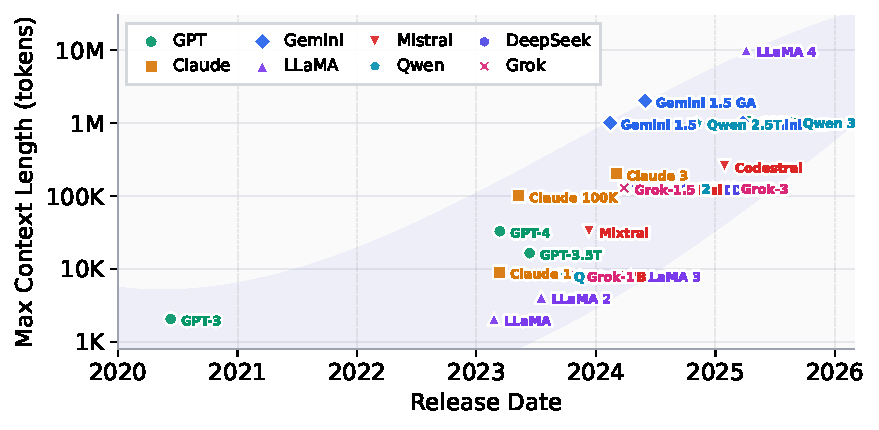
\includegraphics[width=\linewidth]{figure/context_length_evolution.pdf}
  \vspace{-2em}
  \caption{Evolution of maximum model context length across major model families (2020--2026). The shaded band represents the dynamic distribution of model capabilities, showing a rapid expansion in context windows since 2023.}
  \label{fig:context-evolution}
\end{figure}

Modern LLM applications have evolved significantly from simple single-turn queries.
Conversational chatbots now maintain extensive multi-turn histories to provide contextual
and personalized responses, while autonomous system agents operate with massive
system prompts containing detailed instructions, available tool descriptions,
and complex reasoning scratchpads. This evolution has driven the demand for
ever-increasing context windows (as shown in Figure~\ref{fig:context-evolution}). 
For instance, a recent study by OpenRouter~\cite{aubakirova2026state} reveals
that the average sequence length of LLM requests has more than tripled,
growing from under 2,000 tokens in late 2023 to over 5,400 tokens by late 2025.
The same study shows that this trend is even more pronounced for programming
workflows, where sequences routinely exceed 20,000 tokens.
Consequently, the length of prefill requests
has grown substantially, making the prompt processing phase a dominant factor in latency.
Because these long contexts frequently share identical prefixes---such as the 
same grounding documents or system instructions across multiple queries---prefix
caching is highly effective.
In fact, production traces show that the cache hit ratio remains consistently
high.
Experimental evaluations of Mooncake's~\cite{qin2025mooncake} disaggregated
KV Cache show it can theoretically process up to $75\%$ of tokens from cache,
with actual block-level hit ratios routinely exceeding $50\%$ and sometimes
$80\%$ in optimal conditions.
More broadly, production deployments that leverage prefix reuse,
such as Red Hat's llm-d~\cite{hayes2026accelerate},
Character.AI~\cite{characterai2024optimizing}, and agentic frameworks like
Manus~\cite{purav2025manus}, report cache hit rates frequently exceeding
$90\%$ or even $95\%$---reinforcing its necessity.

\subsection{The Shift: MoE and the ``Attention Pressure''} 

Simultaneous to the growth in context length, model architectures have shifted toward
Mixture-of-Experts (MoE) designs (e.g., Mixtral, Qwen-MoE)~\cite{zhou2022mixture, shen2023mixture}.
In dense Transformer models, the Multi-Layer Perceptron (MLP) layers dominate the
parameter count and computation time during the prefill phase. However, MoE architectures
substantially accelerate the MLP stages by activating only a sparse subset of experts
for each token. 

\begin{figure}[t]
  \centering
  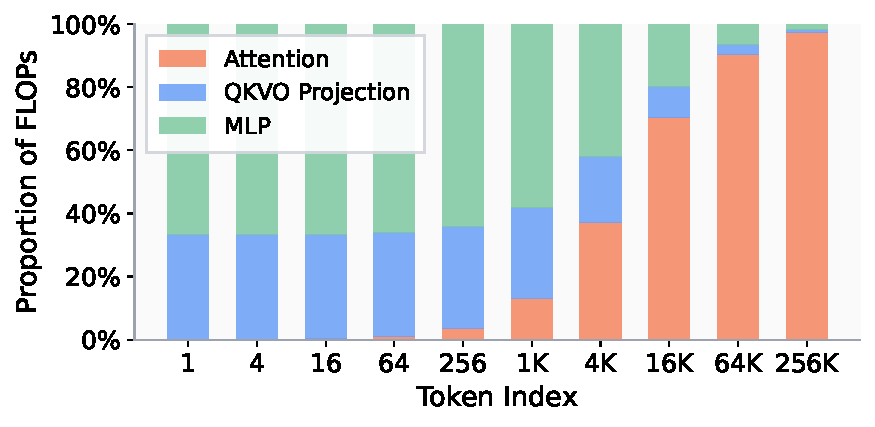
\includegraphics[width=\linewidth]{figure/flop_proportion.pdf}
  \vspace{-2em}
  \caption{Proportion of per-token FLOPs dedicated to Attention, MLP, and QKVO projections during the prefill phase for Qwen3 Coder 30B model~\cite{qwen3technicalreport}. As the sequence length grows, attention rapidly dominates the computational cost.}
  \label{fig:flop-proportion}
  \vspace{-1.5em}
\end{figure}

Because the attention mechanism must still calculate dense interactions
across all tokens in the sequence, the relative cost of attention computation increases
dramatically compared to the MLP projections. Figure~\ref{fig:flop-proportion} illustrates this 
shifting bottleneck for a modern MoE model (Qwen3-Coder-30B-A3B-Instruct~\cite{qwen3technicalreport}). 
While MLP and QKVO projections require a constant number of operations per token, 
the exact self-attention computation scales linearly with the token's position index. 
For deep tokens (e.g., near the 200K limit), the attention mechanism absorbs the 
vast majority of the floating-point operations.
As a result, long-context LLM serving faces immense ``attention pressure'': 
the computational bottleneck of the prefill phase shifts heavily toward the attention layers.

\subsection{The Necessity of Computation-Aware Eviction}

\begin{figure}[t]
  \centering
  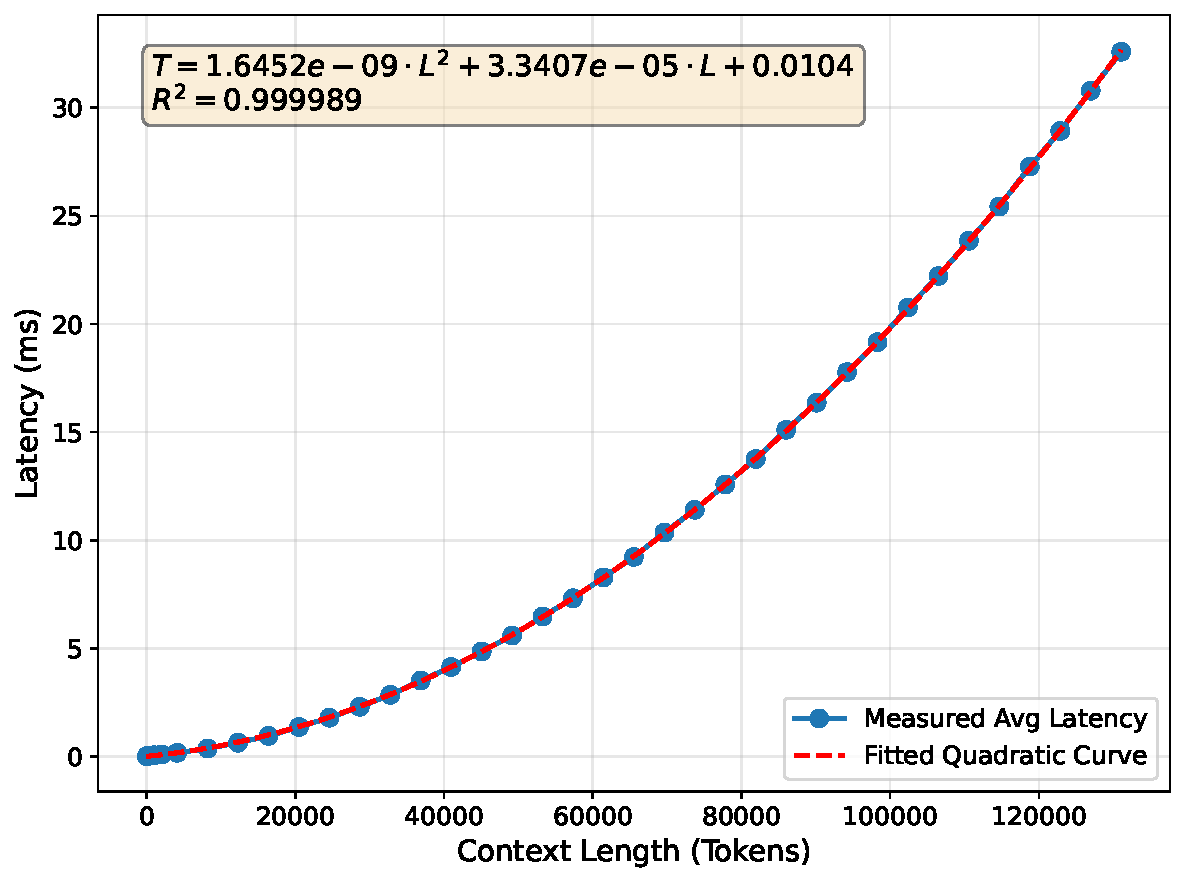
\includegraphics[width=\linewidth]{figure/qwen3_coder_30b_latency_curve.pdf}
  \vspace{-2em}
  \caption{Time-To-First-Token (TTFT) as sequence length increases for a full prefill without prefix cache hits on the Qwen3-Coder-30B model. As shown by the nearly perfect quadratic fit, the execution time scales quadratically rather than linearly, demonstrating the severe latency impact of processing deep tokens and motivating computation-aware eviction.}
  \label{fig:latency-curve}
  \vspace{-1.5em}
\end{figure}

Because of the quadratic arithmetic complexity of exact self-attention ($O(N^2)$),
the computational cost of processing a token is strictly dependent on its position in the
sequence. As shown by the nearly perfect quadratic fit ($R^2=0.999989$) in
Figure~\ref{fig:latency-curve}, the Time-To-First-Token (TTFT) for a full prefill grows
quadratically---not linearly---with sequence length due to this attention overhead.
Recomputing a token deep in the prefix tree (e.g., at index 100,000)
requires calculating dot products with all 99,999 preceding tokens. Conversely,
recomputing a token near the root of the tree requires negligible attention overhead.
Therefore, the blocks at different indices have vastly different recomputation times.

When a structure-agnostic algorithm like LRU treats all cache blocks equally, it
often evicts deep, highly expensive blocks simply because they were least recently used.
The next request that relies on that evicted block will suffer a massive TTFT spike
due to the $O(N^2)$ recomputation penalty. To prevent this, a computation-aware
eviction strategy is critical. By ensuring that blocks requiring the most compute to
regenerate are protected, the system shifts its optimization objective from simply
maximizing naive \textit{cache hit rates} to minimizing \textit{overall computational
overhead}, thereby protecting user experience.

For example, consider the cost of recomputing a sequence of 1,024 tokens using the
Qwen3-Coder-30B-A3B-Instruct model configuration
(from Figure~\ref{fig:flop-proportion}).
If the system must recompute 1,024 tokens at the root of the prefix tree
(indices 0 to 1,023), the total computational cost is approximately 0.13\,TFLOPs.
However, if those same 1,024 tokens are located deep in the context
(starting at index 65,536 (64K)), the required operations skyrocket to 1.22\,TFLOPs.
Because the exact self-attention overhead scales linearly with each token's position,
recomputing a block at a 64K depth is nearly $10\times$ more computationally
expensive than recomputing an equivalent block at the root.
Empirically, this translates directly to severe latency spikes: prefilling a 1K-token
block at the root yields a Time-To-First-Token (TTFT) of only 58\,ms, whereas prefilling
the exact same 1K block after a 64K cached prefix takes 335\,ms---a nearly $6\times$
latency degradation.


\section{Cache Algorithm Design}

Here, we focus on improving the efficiency of the prefix cache algorithm in
terms of computation. In \S\ref{sec:decoupling-tree-with-eviction}, we
have already discussed that the tree structure actually have nothing to do
with the cache eviction, i.e., we can evict not only the leaf nodes, but also
the internal nodes. In this section, we will start with an pessimistic offline
optimal policy, followed by an efficient offline algorithm, and finally
introduce online algorithms.



\subsection{The Pessimistic Offline Optimal Policy}



To dig into the potential of the prefix cache algorithm, we first introduce
our Pessimistic Offline Optimal Policy. The pessimistic offline optimal policy
can be represented by an integer linear programming (ILP) problem.

Let $\mathcal{I}$ be the set of all reuse intervals across the workload. 
A reuse interval $i \in \mathcal{I}$ is defined as the temporal span between
two consecutive accesses to the same block. 
By formulating the variables as reuse intervals, blocks accessed only once
(i.e., one-hit wonders) do not form a closed interval and are naturally
excluded from the problem.
For each reuse interval $i \in \mathcal{I}$, let $c_i$ denote its cost
(e.g., the computation saved if the block is cached) and let $s_i$ be the size
of the block.
We introduce a binary decision variable $x_i \in \{0, 1\}$, where $x_i = 1$ if
the block is kept in the cache for the entire duration of interval $i$, and
$x_i = 0$ otherwise.

The objective is to maximize the total cost of the cached reuse intervals:
\begin{equation}
    \max \sum_{i \in \mathcal{I}} c_i x_i.
\end{equation}

Traditionally, a cache must enforce a capacity check at every fine-grained
execution step.
However, this introduces an excessive number of constraints.
To ensure space availability while keeping the formulation computationally
tractable, our policy evaluates the capacity constraint \emph{only before the
first block of each request}. 

Let $\mathcal{R}$ be the set of all requests, where each request
$r \in \mathcal{R}$ starts at time $t_r$ and has a length (or size) of $L_r$.
Let $\mathcal{I}_r \subseteq \mathcal{I}$ be the set of reuse intervals that
are active precisely at time $t_r$ (i.e., the interval spans across the arrival
of the request, $\text{start}_i \le t_r < \text{end}_i$).
The cache capacity constraint dictates that right before executing the request,
the sum of all cached blocks plus the length of the incoming request must not
exceed the cache capacity:
\begin{equation}
    \sum_{i \in \mathcal{I}_r} s_i x_i + L_r \le C \quad \forall r \in \mathcal{R},
\end{equation}
where $C$ is the cache capacity limit. 

This formulation is termed \emph{pessimistic} because it assumes a worst-case
space requirement.
By forcing the cache to hold all currently active intervals \emph{and} the
entire length of the incoming request simultaneously at the start of the request,
we ignore the fact that in a real execution, some blocks could be evicted
mid-request, or the request's tokens are consumed/generated sequentially
rather than taking up the full $L_r$ capacity all at once.
While providing a strict lower bound on what can be safely cached without
out-of-memory errors, performing the capacity check exclusively before
serving the first block ensures sufficient space is allocated up front and
significantly reduces the number of constraints in the ILP solver.

\subsection{Efficient Offline Algorithm: Belady Compute}

Despite the optimization largely reducing the number of constraints, the ILP
problem is still computationally expensive. To address this, we introduce
Belady Compute, an efficient offline algorithm that approximates the optimal
solution.

The Belady Compute algorithm is inspired by the same fundamental idea as
Belady's algorithm~\cite{belady1966study, mattson1970evaluation}
(or Belady Size in variable-size caching), which evicts the
item that will be needed furthest in the future. To account for the
heterogeneous computation cost of prefix cache blocks, Belady Compute adapts
this metric by normalizing the future distance by the block's computation cost.

Specifically, when a cache eviction is required, Belady Compute selects the
block that maximizes the following eviction metric:
\begin{equation}
    \text{Eviction Metric} = \frac{\text{Time to next access}}{\text{Computation cost}}.
\end{equation}
Here, the \emph{time to next access} is measured discretely in terms 
of the number of incoming KV cache block requests before the block is
accessed again, and the \emph{computation cost} is the computation overhead
that would be incurred if the block were evicted and needed to be recomputed.
By evicting the block with the highest value of this metric, the algorithm
prioritizes retaining blocks that will be reused soon and those that are
highly expensive to recompute.



\subsection{\algo{}: \algofull{} Algorithm}

We have also designed an online algorithm, \algofull Algorithm (\algo),
which prioritizes simplicity and low implementation overhead. Unlike complex
predictive policies, \algo is a straightforward online policy that requires
minimal state—only a per-block access counter and a last-access timestamp.

To balance frequency, recency, and computation costs without manual parameter
tuning, \algo evaluates blocks using a single unified metric. When an
eviction is triggered, \algo selects the block $b$ that minimizes:
\begin{equation}
    \text{Eviction Metric}(b) = \frac{\text{Frequency}'(b) \cdot C(b)}{\text{Recency}(b)},
\end{equation}
where $\text{Frequency}'(b)$ is the adjusted access frequency, $\text{Recency}(b)$ is
the time since the last access (e.g., measured in request counts), and $C(b)$
is the computation cost.

To protect the cache from being polluted by blocks that are accessed only once (i.e., ``one-hit wonders''), \algo implements a \textit{quick demotion} mechanism. If a block has only been accessed once ($\text{Frequency}(b) = 1$), its priority is significantly reduced by applying a penalty factor (e.g., $\text{Frequency}'(b) = 0.1$). For all other blocks, the adjusted frequency is equal to the actual access count ($\text{Frequency}'(b) = \text{Frequency}(b)$).

This simple ratio inherently implements an aging mechanism: a historically
popular block's priority naturally decays as it remains idle. By scaling
the metric by $C(b)$ and applying the quick demotion penalty, \algo efficiently 
retains expensive-to-compute blocks while allowing active, recently accessed 
sequences to replace stale or transient ones. This approach provides a 
practical, low-overhead solution for computation-aware prefix caching.


\section{System Design}

In this section, we present \sys (\sysfull), a system that efficiently
manages prefix-matched KV caches while addressing the performance impact of
fragmentation. We first analyze the impact of ``holes'' in the KV cache
(\S\ref{sec:hole-analysis}) and then detail our hole-aware algorithm design
(\S\ref{sec:hole-aware-algorithm-design}). Finally, we describe the
implementation of \sys in vLLM.

\subsection{Hole Analysis: Minimal Acceptable Overhead for Each Hole}
\label{sec:hole-analysis}

As discussed in Section~\ref{sec:decoupling-tree-with-eviction}, the logical
structure of the prefix tree is physically decoupled from cache eviction.
Because we evict the KV cache on a physical block basis rather than at the
granularity of entire sequences or tree nodes, some intermediate blocks within
a cached prefix may be evicted while surrounding blocks remain in memory. This
block-level eviction natively creates ``holes'' in the cached sequence.
Furthermore, for sample-based eviction algorithms, the probabilistic nature
of sampling can exacerbate this effect, potentially causing hundreds of
holes within a single sequence.
% Nevertheless, this approach remains correct:
% the logical dependencies of the prefix tree are preserved, and the system
% can simply recompute any missing blocks (the holes) during the prefill
% phase without invalidating subsequent cached blocks.

Small holes make the prefill less efficient.
This is primarily because the scheduling overhead is small compared to the small
prefill time that each hole results in.
Therefore, a hole-aware eviction and allocation algorithm is strictly necessary.
When limited to a few large holes, caching fragmented blocks rescues massive
computational cost.
However, if an unmanaged or sample-based eviction policy randomly scatters
hundreds of microscopic holes across the context, the accumulated prefill
time for these microscopic holes will completely negate any attention scaling
savings.
Thus, a successful hole-aware design must maximize cache reuse while explicitly
bounding the total number of fragmentation holes.

\subsection{Hole-aware Algorithm Design}
\label{sec:hole-aware-algorithm-design}

To implement a hole-aware caching strategy that bounds fragmentation while
providing efficient eviction, \sys builds a radix tree structure in memory.
This allows us to track the physical blocks for cached prefixes and sample
on the radix tree nodes directly rather than on individual blocks.
The core principle of our approach is to try evicting continuous blocks within
the same node. By prioritizing the eviction of contiguous blocks instead of
randomly scattering victims, we naturally avoid severe fragmentation and
minimize the number of holes created in the cache.

Every time eviction is triggered, we sample a subset of candidate nodes. We pick
one canonical block from each node to calculate its eviction score (e.g.,
based on the frequency-aging metric from our \algo algorithm). Once a victim
node is selected based on
these scores, we attempt to evict blocks sequentially from the beginning of the
node to its end. Finally, if all blocks in the node are evicted and it becomes
a leaf node, we prune it from the radix tree.

The high-level eviction protocol operates in a tiered priority to minimize the
disruptive impact of holes. As described in Algorithm~\ref{alg:eviction}, we
systematically search for evictable blocks through the following ordered stages, 
accumulating freed blocks ($E$) until the requested limit ($N$) is satisfied:
\begin{enumerate}
    \item \textbf{Unhashed blocks queue~($\mathcal{Q}_{\text{unhashed}}$):}
    We first pop from the unhashed blocks queue to evict blocks that do not
    have hashes, which include non-full blocks and free blocks.
    \item \textbf{Blocks not in tree~($\mathcal{Q}_{\text{not-in-tree}}$):}
    Next, we pop blocks that are fully formed but not linked into the
    tree~(e.g., blocks created during speculative decoding that were ultimately
    not accepted).
    \item \textbf{Free radix tree nodes~($\mathcal{S}_{\text{Free}}$):}
    Then we sample a candidate subset of $k_{\text{sample}}$ free radix tree
    nodes ($\mathcal{V}_{\text{sample}}$) from the free node list
    $\mathcal{S}_{\text{Free}}$ that are not currently referenced by any
    running requests. We model an eviction score ($\Call{Score}{v}$, e.g.,
    representing hotness) such that the lowest score is better for eviction,
    and select the candidate $v^*$ with the lowest score, sequentially
    evicting blocks within it.
    \item \textbf{In-use radix tree nodes~($\mathcal{S}_{\text{InUse}}$):}
    As a last resort, we sample and evict from the in-use radix tree node list
    $\mathcal{S}_{\text{InUse}}$ similarly. While most blocks are referenced
    by running requests (i.e., unevictable), unreferenced portions of them may
    sometimes be evicted.
\end{enumerate}

\begin{algorithm}[htbp]
\small
\caption{Hole-aware Eviction Logic}
\label{alg:eviction}
\begin{algorithmic}[1]
% \Require Target number of blocks to evict $N$
\Procedure{EvictBlocks}{$N$}
    \State $E \gets 0$ 
    \State \Comment{1. Try to get free blocks from unhashed queue}
    \State $E \gets E + {}$\Call{EvictFromQueue}{$\mathcal{Q}_{\text{unhashed}}$, $N - E$}
    \If{$E = N$}~ \textbf{return} $N$ \EndIf
    \State \Comment{2. Try to get free blocks from blocks not in tree}
    \State $E \gets E + {}$\Call{EvictFromQueue}{$\mathcal{Q}_{\text{not-in-tree}}$, $N - E$}
    \If{$E = N$}~ \textbf{return} $N$ \EndIf
    \State \Comment{3. Try to get free blocks from free radix tree nodes}
    \State $E \gets E + \Call{EvictFromNodes}{\mathcal{S}_{\text{Free}}, N - E}$
    \If{$E = N$}~ \textbf{return} $N$ \EndIf
    \State \Comment{4. Try to get free blocks from in-use radix tree nodes}
    \State $E \gets E + \Call{EvictFromNodes}{\mathcal{S}_{\text{InUse}}, N - E}$
    \State \textbf{return} $E$
\EndProcedure
\Statex
\Function{EvictFromQueue}{$\mathcal{Q}$, $M$}
    \State $k \gets \min(M, |\mathcal{Q}|)$
    \State \Call{Pop}{$\mathcal{Q}$, $k$}
    \State \textbf{return} $k$
\EndFunction
\Statex
\Function{EvictFromNodes}{$\mathcal{S}$, $M$}
    \State $E \gets 0$
    \While{$E < M$ \textbf{and} $\mathcal{S} \neq \emptyset$}
        \State $\mathcal{V}_{\text{sample}} \gets \Call{SampleNodes}{\mathcal{S}, k_{\text{sample}}}$
        \If{$\mathcal{V}_{\text{sample}} = \emptyset$}~ \textbf{break} \EndIf
        \State $v^* \gets \mathop{\mathrm{argmin}}_{v \in \mathcal{V}_{\text{sample}}} \Call{Score}{v}$
        \State $E \gets E + {}$\Call{EvictBlocksFromNode}{$v^*$, $M - E$}
    \EndWhile
    \State \textbf{return} $E$
\EndFunction
\Statex
\Function{EvictBlocksFromNode}{$v$, $M$}
    \State $E \gets 0$
    \For{$b \in v$}
        \If{$E = M$}~ \textbf{break} \EndIf
        \If{$b$ in memory \textbf{and} $b.ref\_cnt = 0$}
            \State \Call{Evict}{$b$}; $E \gets E + 1$
        \EndIf
    \EndFor
    \If{$v$ is leaf node \textbf{and} $v$ is empty}
        \State \Call{Prune}{$v$}
    \EndIf
    \State \textbf{return} $E$
\EndFunction
\end{algorithmic}
\end{algorithm}

\subsection{Implementation}
\label{sec:implementation}

We implemented \sys in vLLM~\cite{kwon2023efficient}.
Because the original codebase assumes prefix matching is strictly contiguous
and prefix-only, we introduced several abstraction layers to facilitate
segmented prefix matching.

When a request arrives, the system performs a maximal segmented match against
the radix tree to identify all reusable prefix segments. This matching process
produces a list of \texttt{KVCacheBlockSegment} objects, each representing a
sequence of contiguous blocks found in the cache. Once identified, these
segments are immediately referenced to prevent eviction during the execution
cycle.

\begin{figure}[t]
  \centering
  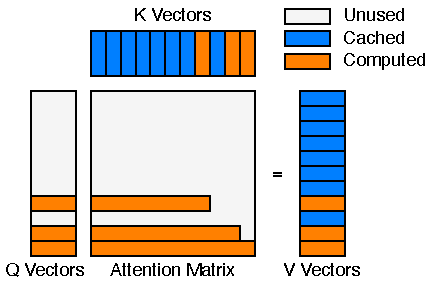
\includegraphics[width=\linewidth]{figure/hole_filling.pdf}
  \vspace{-2em}
  \caption{Batched hole-filling implementation. Instead of sequential processing, \sys aggregates all missing tokens to compute QKV projections and attention in parallel, minimizing scheduling overhead.}
  \label{fig:hole-filling}
\end{figure}

To handle the gaps between these hits, \sys implements an optimized hole-filling 
mechanism. Rather than filling holes sequentially in multiple rounds, we 
exploit the lack of dependencies between disparate missing segments when 
the surrounding context is already cached. As shown in 
Figure~\ref{fig:hole-filling}, the system calculates the QKV projections for all 
tokens belonging to any hole simultaneously. It then computes the parts 
of the attention matrix corresponding to these holes in a single batched operation. 
By processing all holes together, we significantly reduce scheduling 
overhead and kernel launch latency, ensuring that fragmented cache hits 
remain computationally efficient. In the event of preemption, the system safely 
unreferences both the integrated sequences and any pending hit segments that 
have yet to be processed, ensuring memory is correctly reclaimed.

Additionally, we developed a new abstraction layer for block management that
replaces the original design, which was strictly tied to an LRU policy. This
framework enables granular tracking of block access patterns and maintains a
radix tree to support diverse eviction policies. Using this architecture, we
implemented Belady-Compute, and \algo{} with the
hole-aware algorithm design detailed in \S\ref{sec:hole-aware-algorithm-design}.


\section{Evaluation}

\subsection{Evaluation Setup}
\label{sec:evaluation-setup}

\pgheading{Hardware and Software Environment}
All experiments are conducted on a server equipped with an NVIDIA RTX PRO 6000 Blackwell GPU and an AMD Ryzen Threadripper PRO 7975WX 32-Core CPU. We implement \sys on top of the vLLM~\cite{kwon2023efficient} serving engine. Our implementation replaces the default LRU-based prefix caching manager with the hole-aware management system and \algo algorithm described in Section~\ref{sec:implementation}.

\pgheading{Model Configuration}
We use the Qwen3-Coder-30B-A3B-Instruct model~\cite{qwen3technicalreport} for all evaluations. This model follows a Mixture-of-Experts (MoE) architecture, which exhibits significant attention pressure at long context lengths. The model is served using 16-bit precision and is configured with a KV cache block size of 16 tokens.

\pgheading{Workloads and Traces}
To evaluate \sys under realistic serving conditions, we utilize four production traces from the Qwen-Bailian usage dataset~\cite{qwen_bailian_traces}. These traces represent diverse real-world usage patterns including multi-turn conversations, code assistant tasks, and long-context retrieval queries. For each trace, we replay the requests and measure the Time-to-First-Token (TTFT), decoding throughput, and cache hit ratios.
\subsection{Cache Analysis}
\label{sec:cache-analysis}

We evaluate the computational efficiency of \sys across the four production traces described in Section~\ref{sec:evaluation-setup}. Figure~\ref{fig:qwen-cache-analysis} shows the cumulative computation saved (normalized to the total prefill FLOPs) as the cache capacity increases for each workload.

\begin{figure*}[t]
    \centering
    \begin{subfigure}{0.48\textwidth}
        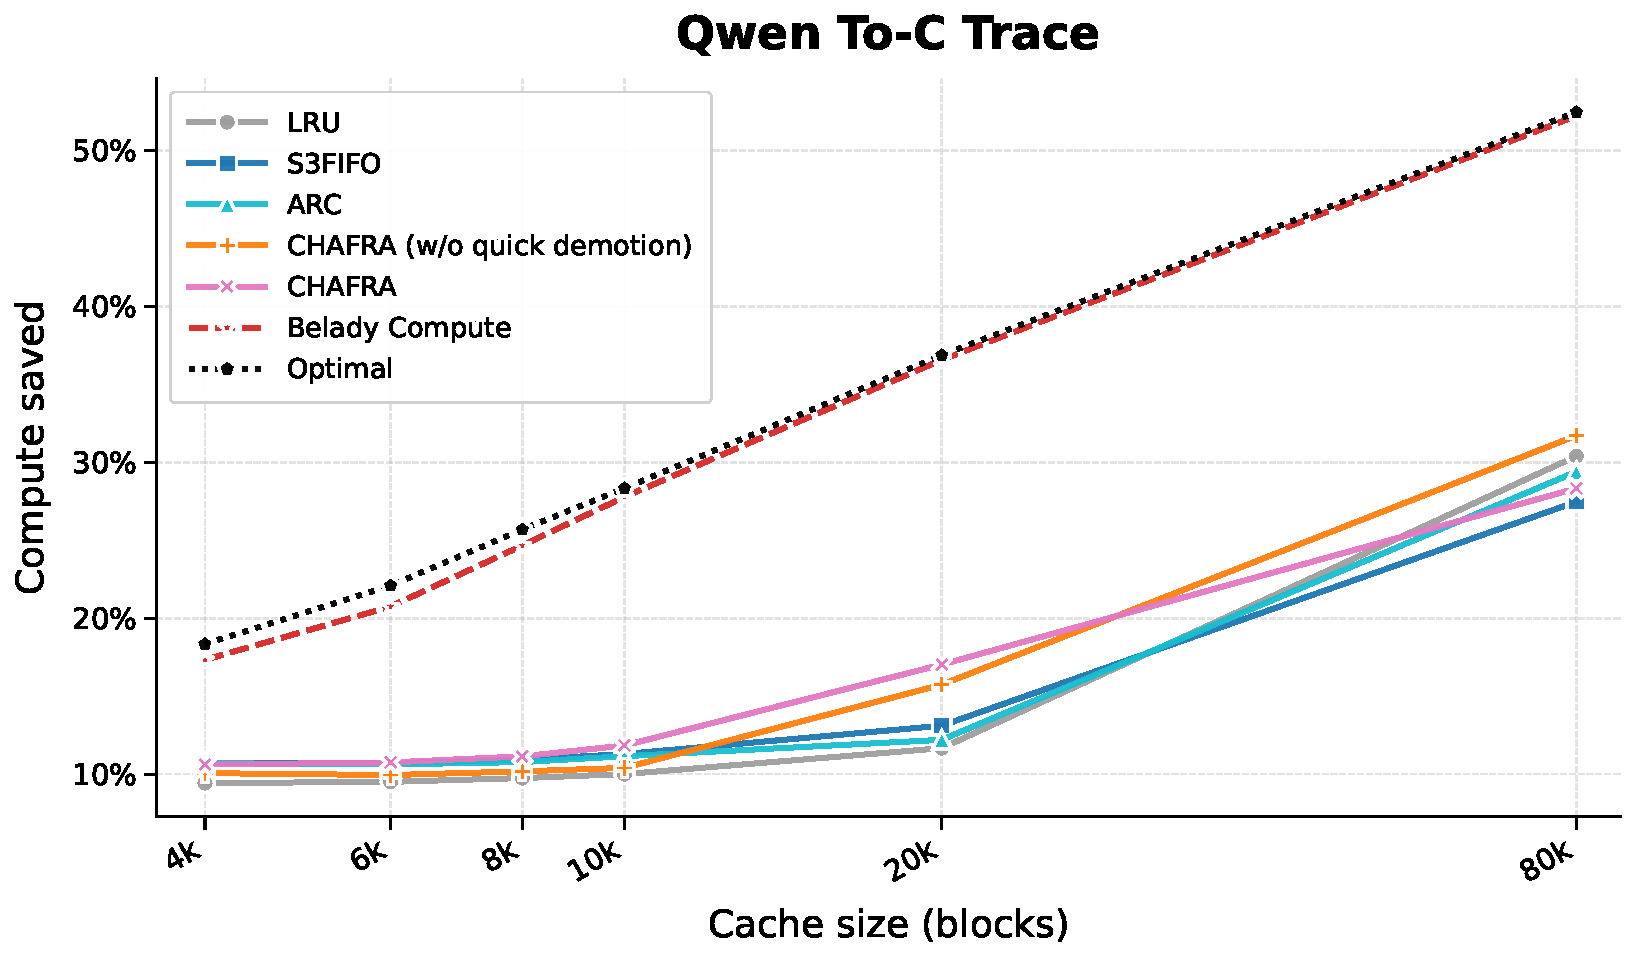
\includegraphics[width=\linewidth]{figure/qwen_traceA_blksz_16_pos_pretty.pdf}
        \caption{General Chat (Trace A)}
        \label{fig:trace-a}
    \end{subfigure}
    \hfill
    \begin{subfigure}{0.48\textwidth}
        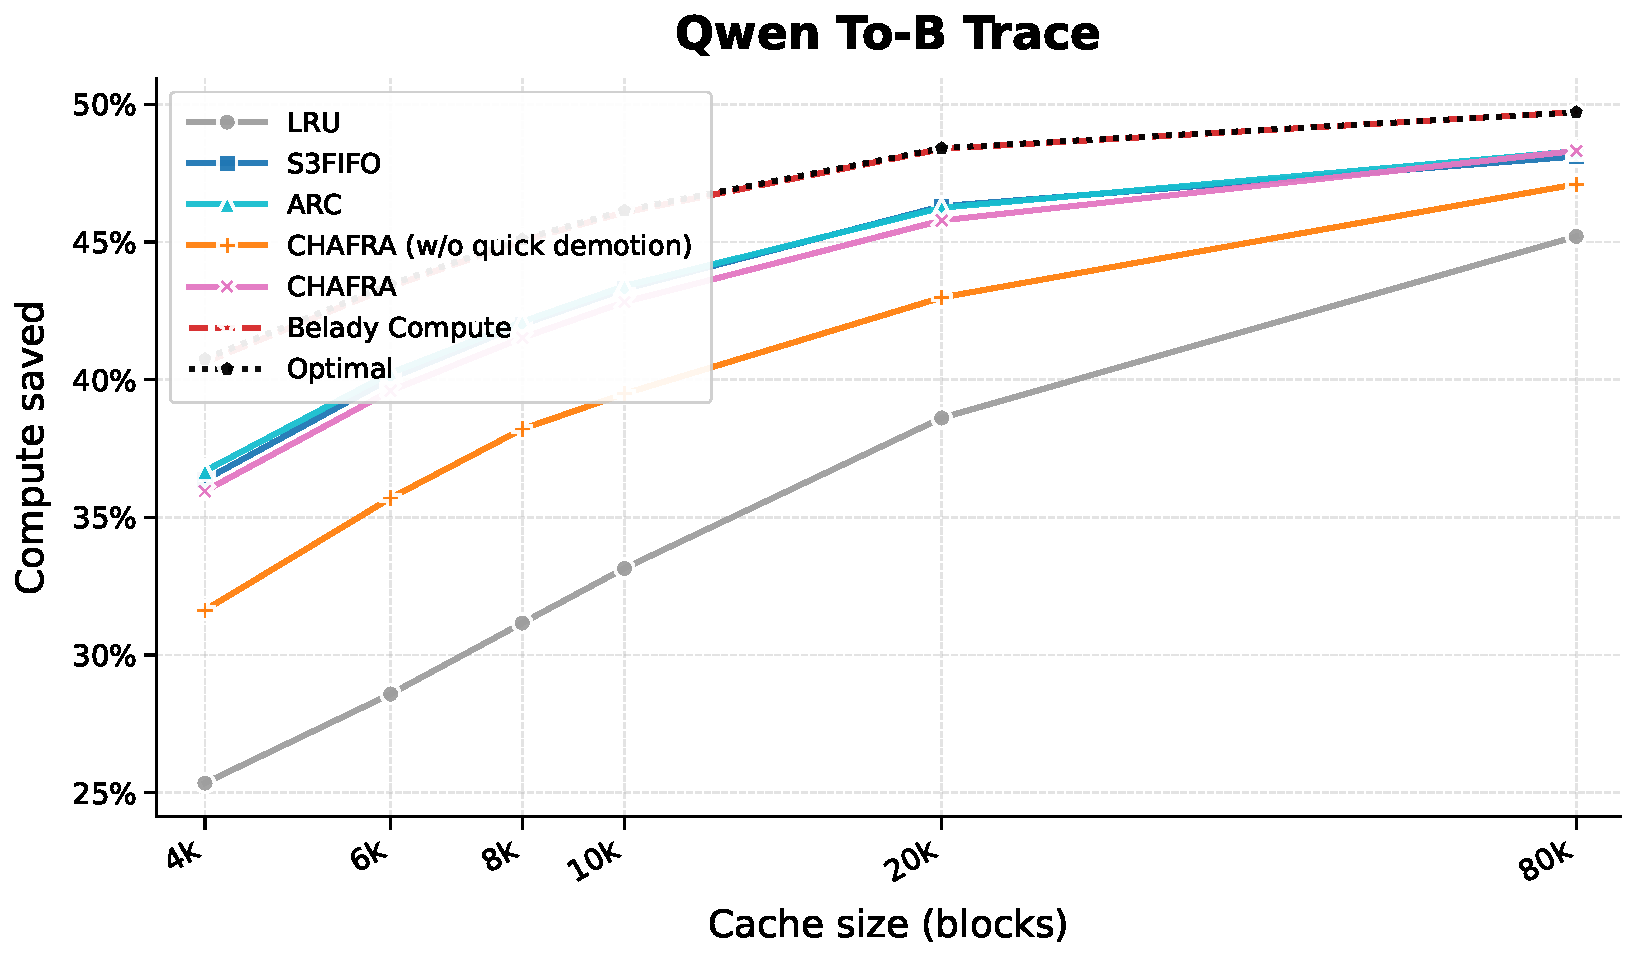
\includegraphics[width=\linewidth]{figure/qwen_traceB_blksz_16_pos_pretty.pdf}
        \caption{Long Retrieval (Trace B)}
        \label{fig:trace-b}
    \end{subfigure}
    
    \vspace{1em}
    
    \begin{subfigure}{0.48\textwidth}
        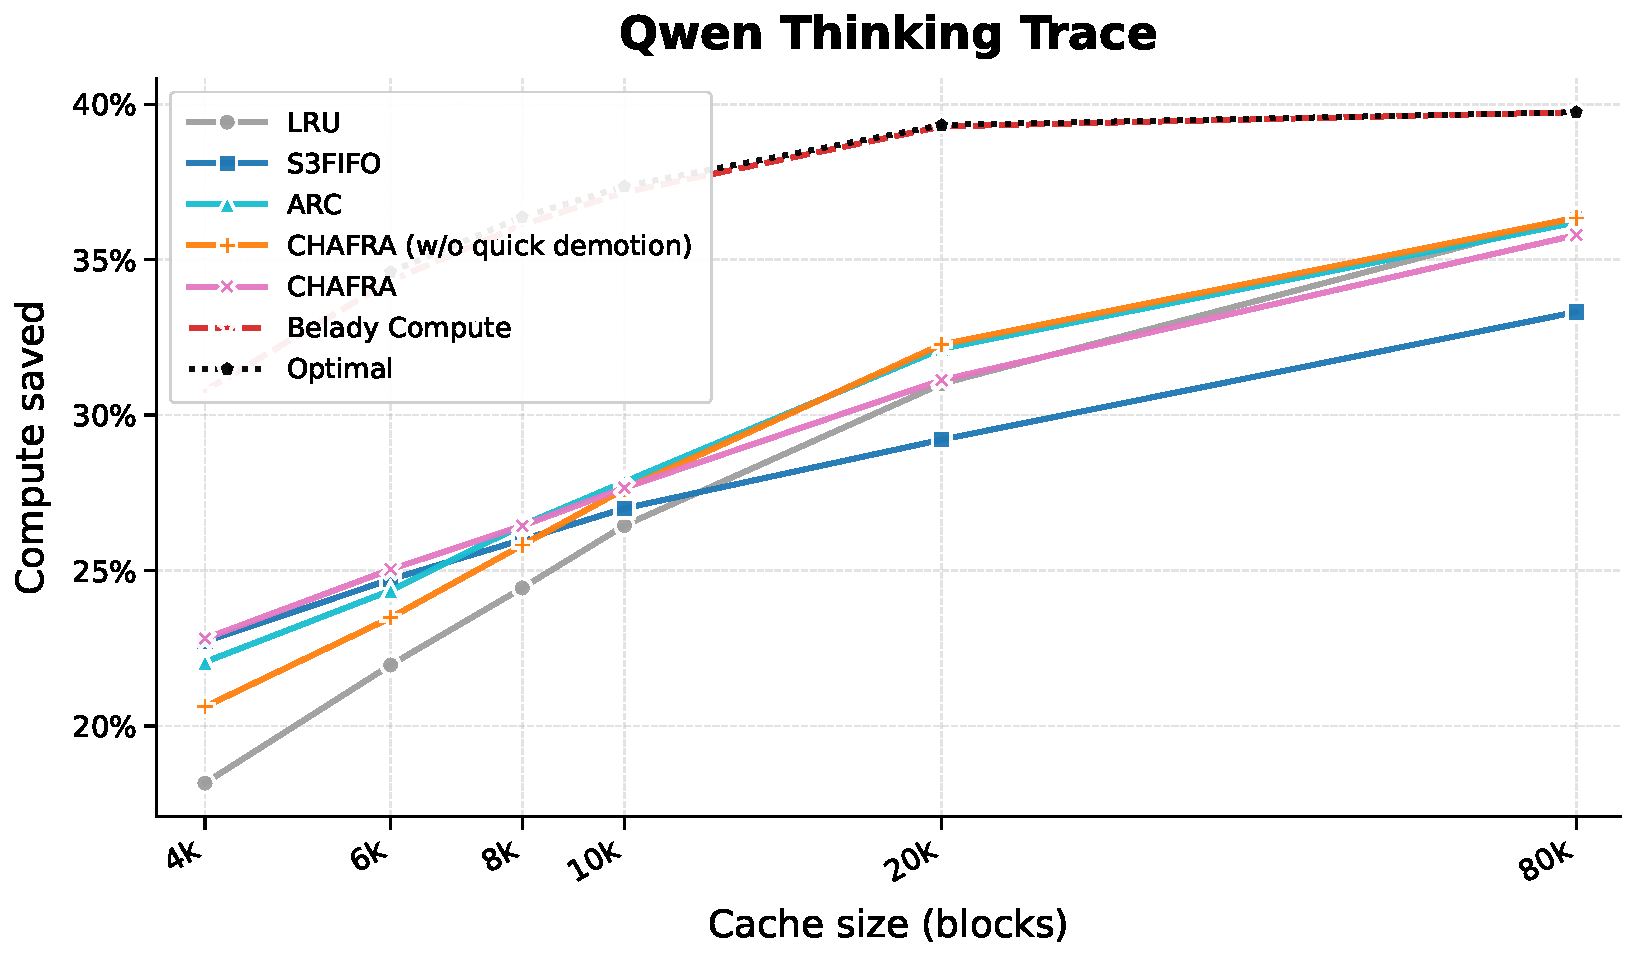
\includegraphics[width=\linewidth]{figure/qwen_thinking_blksz_16_pos_pretty.pdf}
        \caption{Reasoning (Thinking)}
        \label{fig:trace-thinking}
    \end{subfigure}
    \hfill
    \begin{subfigure}{0.48\textwidth}
        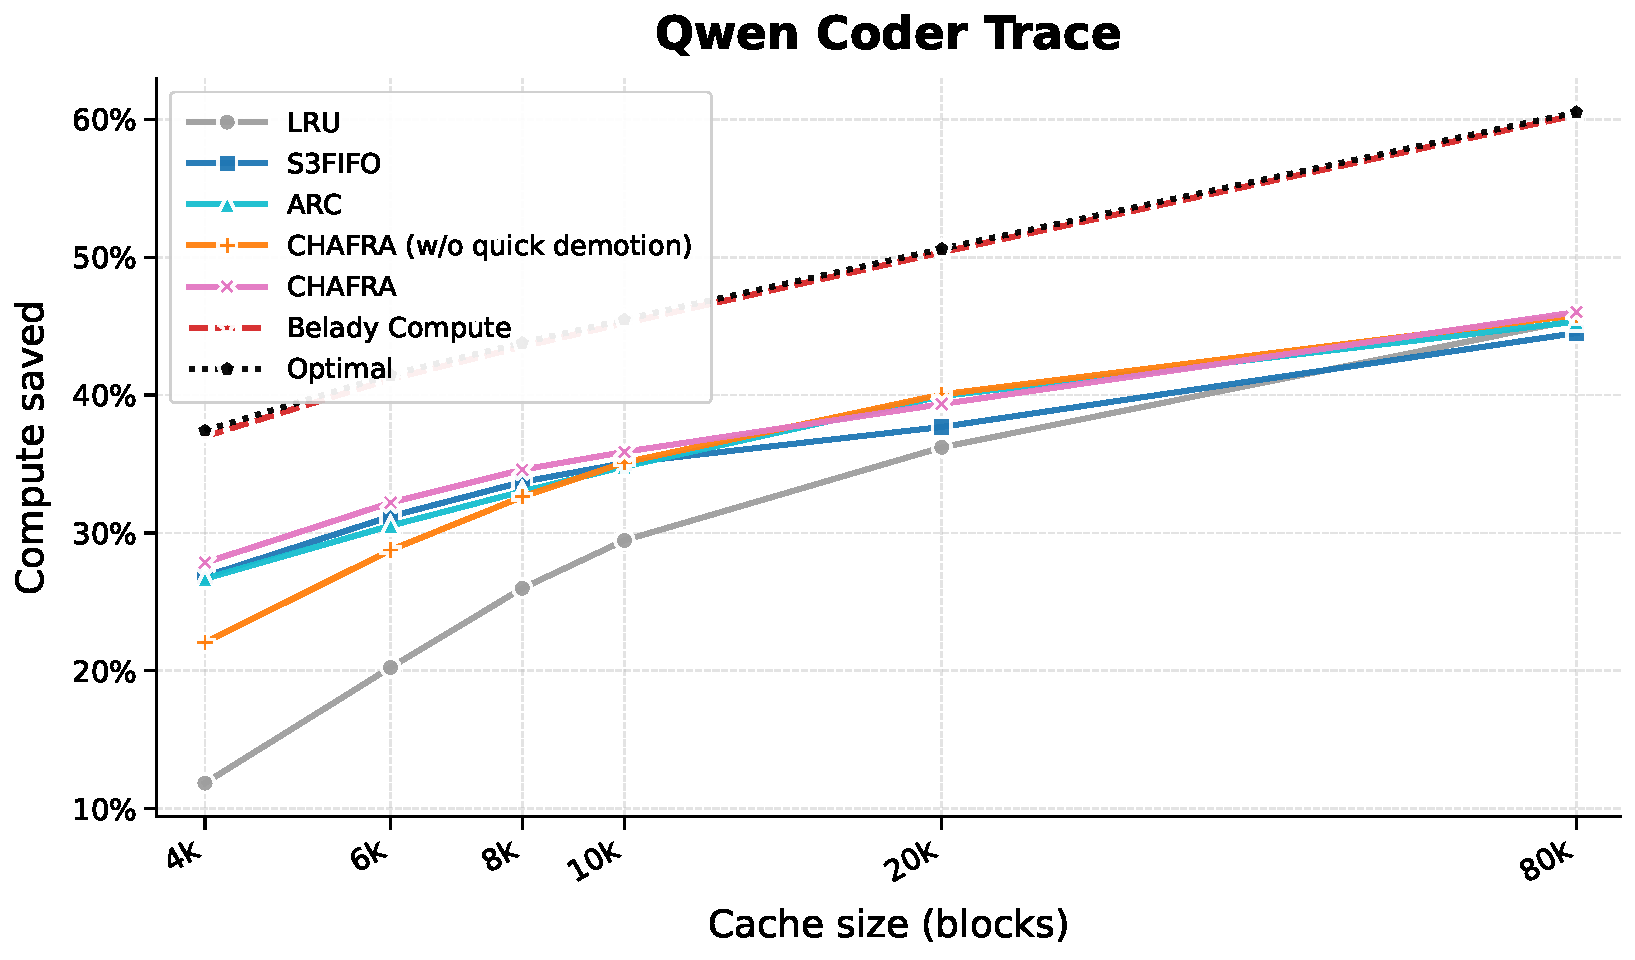
\includegraphics[width=\linewidth]{figure/qwen_coder_blksz_16_pos_pretty.pdf}
        \caption{Coding Assistant (Coder)}
        \label{fig:trace-coder}
    \end{subfigure}
    \caption{Cumulative computational savings across different cache sizes for four Qwen-Bailian traces. \sys (\algo) consistently outperforms LRU and closely follows the Belady-Compute heuristic and the Offline Optimal (ILP).}
    \label{fig:qwen-cache-analysis}
\end{figure*}

\pgheading{Performance of Eviction Policies}
Across all traces, the standard LRU policy exhibits the lowest computational savings. This is because LRU treats all cache blocks as having equal value, frequently evicting deep blocks that are extremely expensive to recompute simply because they have not been accessed recently. In contrast, our proposed online algorithm, \algo, significantly outperforms LRU by explicitly protecting these high-value, deep blocks. By incorporating the recomputation cost $C(b)$ into the eviction metric, \algo ensures that the most computationally intensive portions of the prefix tree remain in the cache.

\pgheading{Near-Optimality of Heuristics}
A key observation from Figure~\ref{fig:qwen-cache-analysis} is that the Belady-Compute heuristic serves as an excellent approximation of the Pessimistic Offline Optimal (ILP) policy. In all four workloads, the performance curve for Belady-Compute is nearly indistinguishable from the ILP solution. This result validates our strategy of normalizing the time-to-next-access by the computation cost, demonstrating that it effectively captures the optimal trade-off between temporal locality and recomputation overhead.

\pgheading{System Improvements}
\sys achieves the most significant gains in the coding trace (Figure~\ref{fig:trace-coder}), where prefix trees are deeper and attention pressure is more acute. In contrast, for traces with less pronounced prefix reuse or shorter shared contexts, such as the reasoning trace (Figure~\ref{fig:trace-thinking}), the benefits of computation-aware eviction are more subtle, though \sys still maintains a lead over the LRU baseline. These results confirm that a computation-aware and hole-aware design is most effective in workloads with high attention pressure, as it shifts the system's optimization goal from simple cache hits to overall computational efficiency.
\subsection{Latency}
\label{sec:latency}

We further evaluate the impact of \sys on the Time-to-First-Token (TTFT) latency. Figure~\ref{fig:qwen-latency-analysis} illustrates the average TTFT across different cache capacities for the four traces.

\begin{figure*}[t]
    \centering
    \begin{subfigure}{0.48\textwidth}
        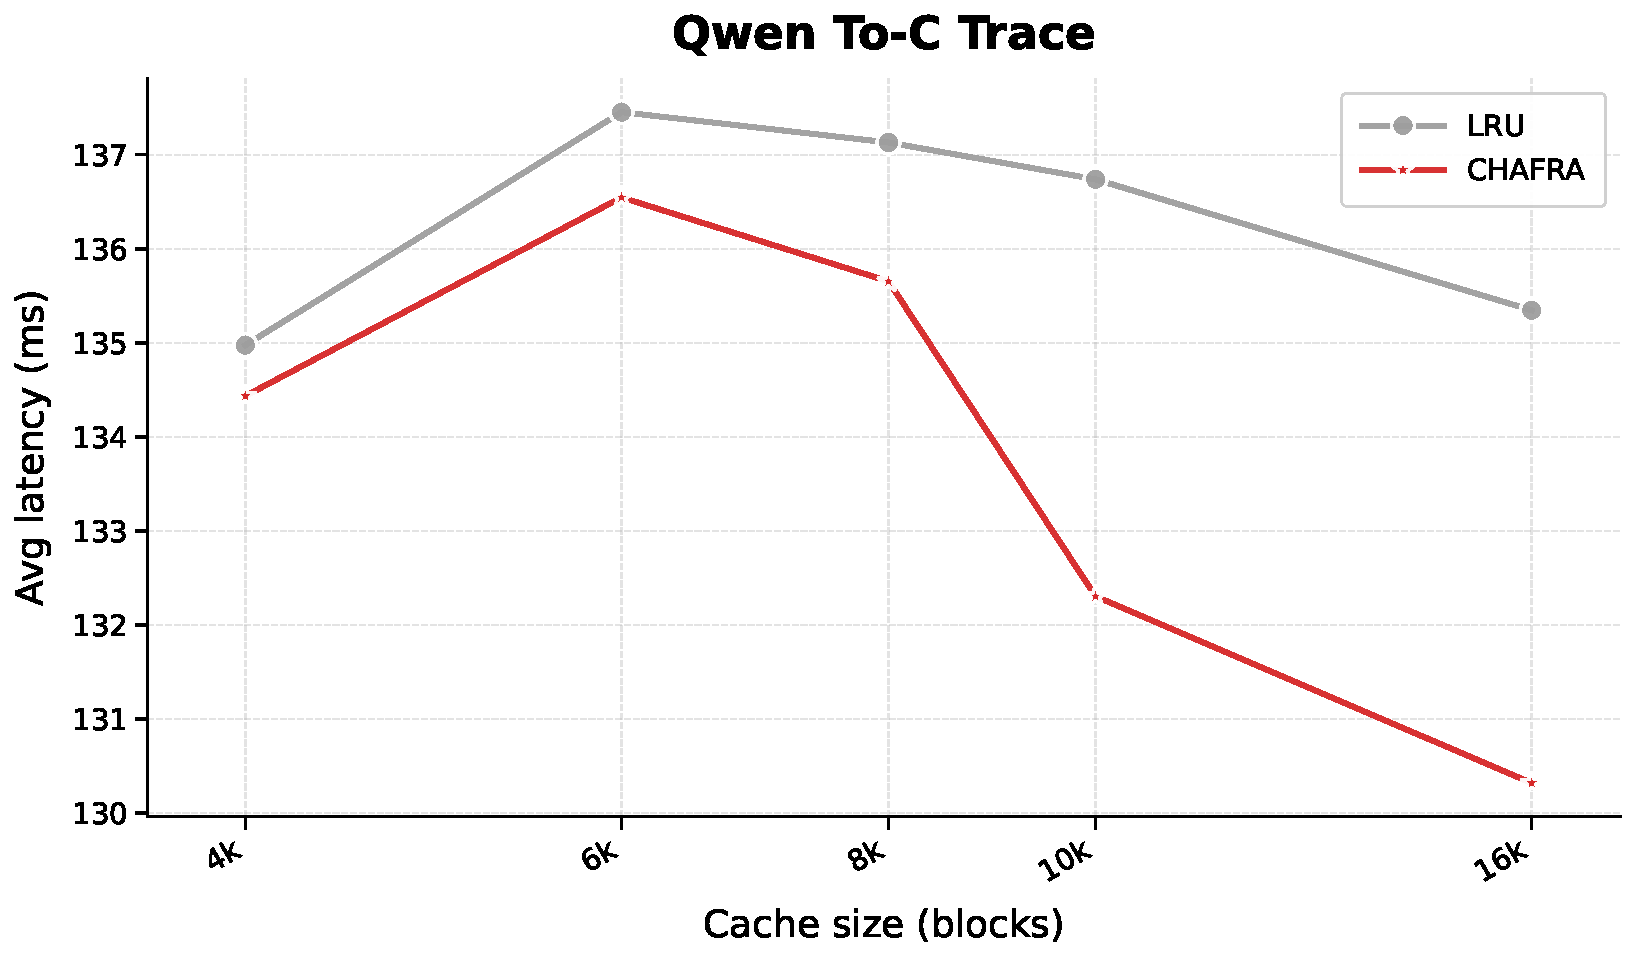
\includegraphics[width=\linewidth]{figure/qwen_traceA_blksz_16_pos_latency_pretty.pdf}
        \caption{General Chat (Trace A)}
        \label{fig:latency-trace-a}
    \end{subfigure}
    \hfill
    \begin{subfigure}{0.48\textwidth}
        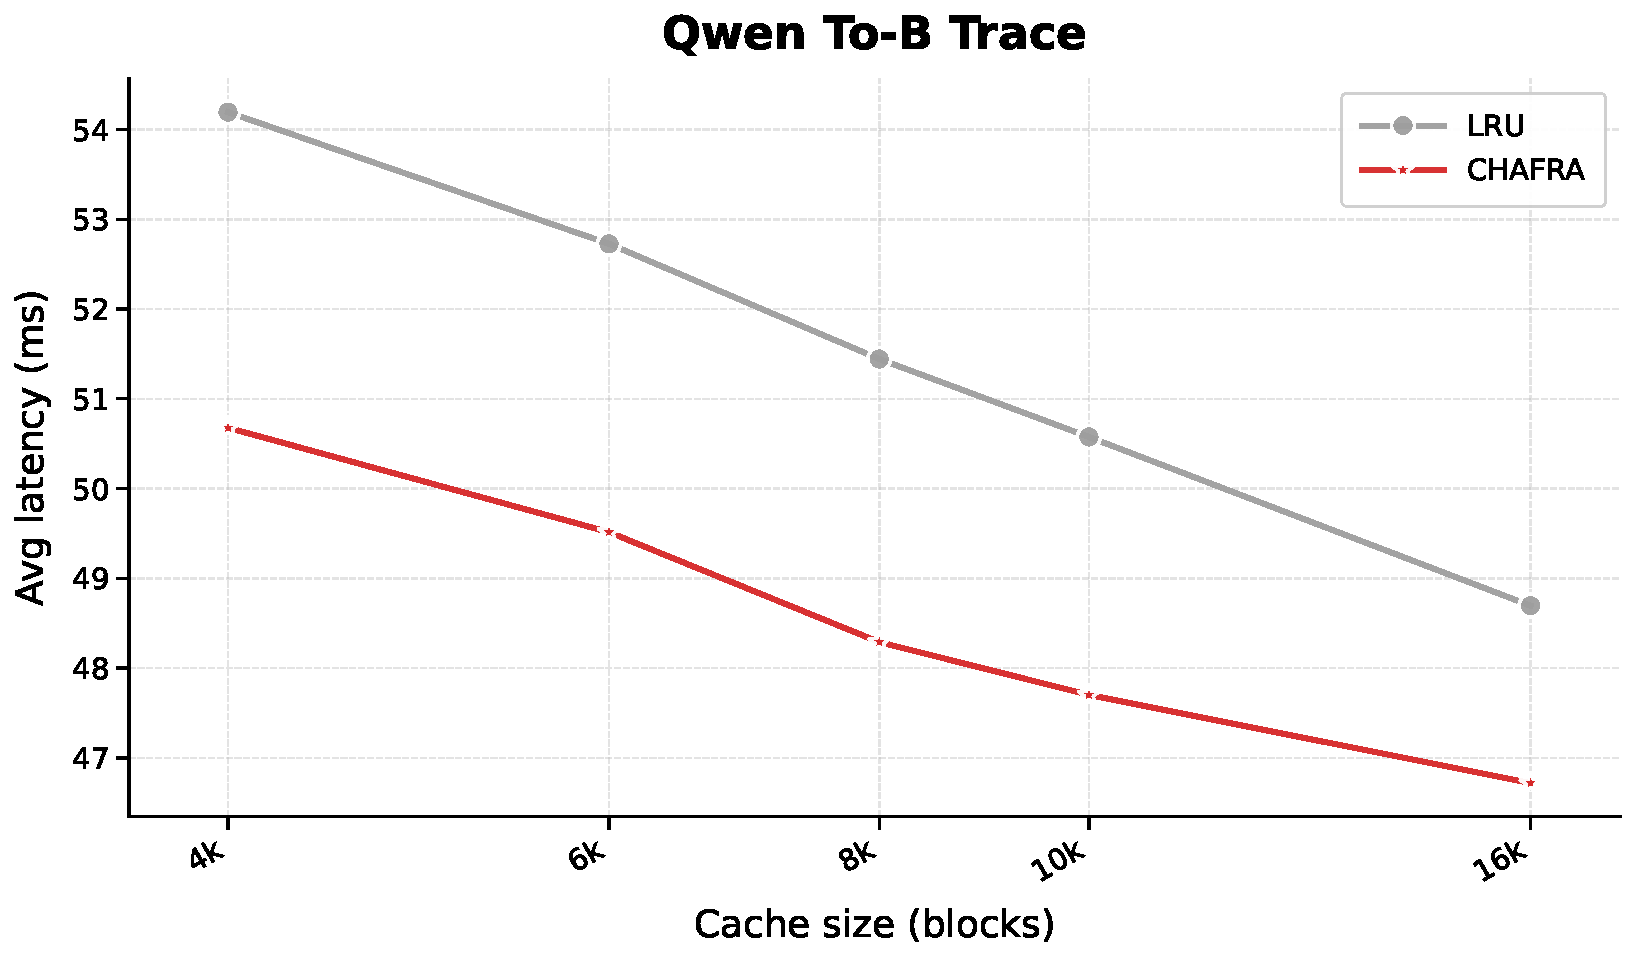
\includegraphics[width=\linewidth]{figure/qwen_traceB_blksz_16_pos_latency_pretty.pdf}
        \caption{Long Retrieval (Trace B)}
        \label{fig:latency-trace-b}
    \end{subfigure}
    
    \vspace{1em}
    
    \begin{subfigure}{0.48\textwidth}
        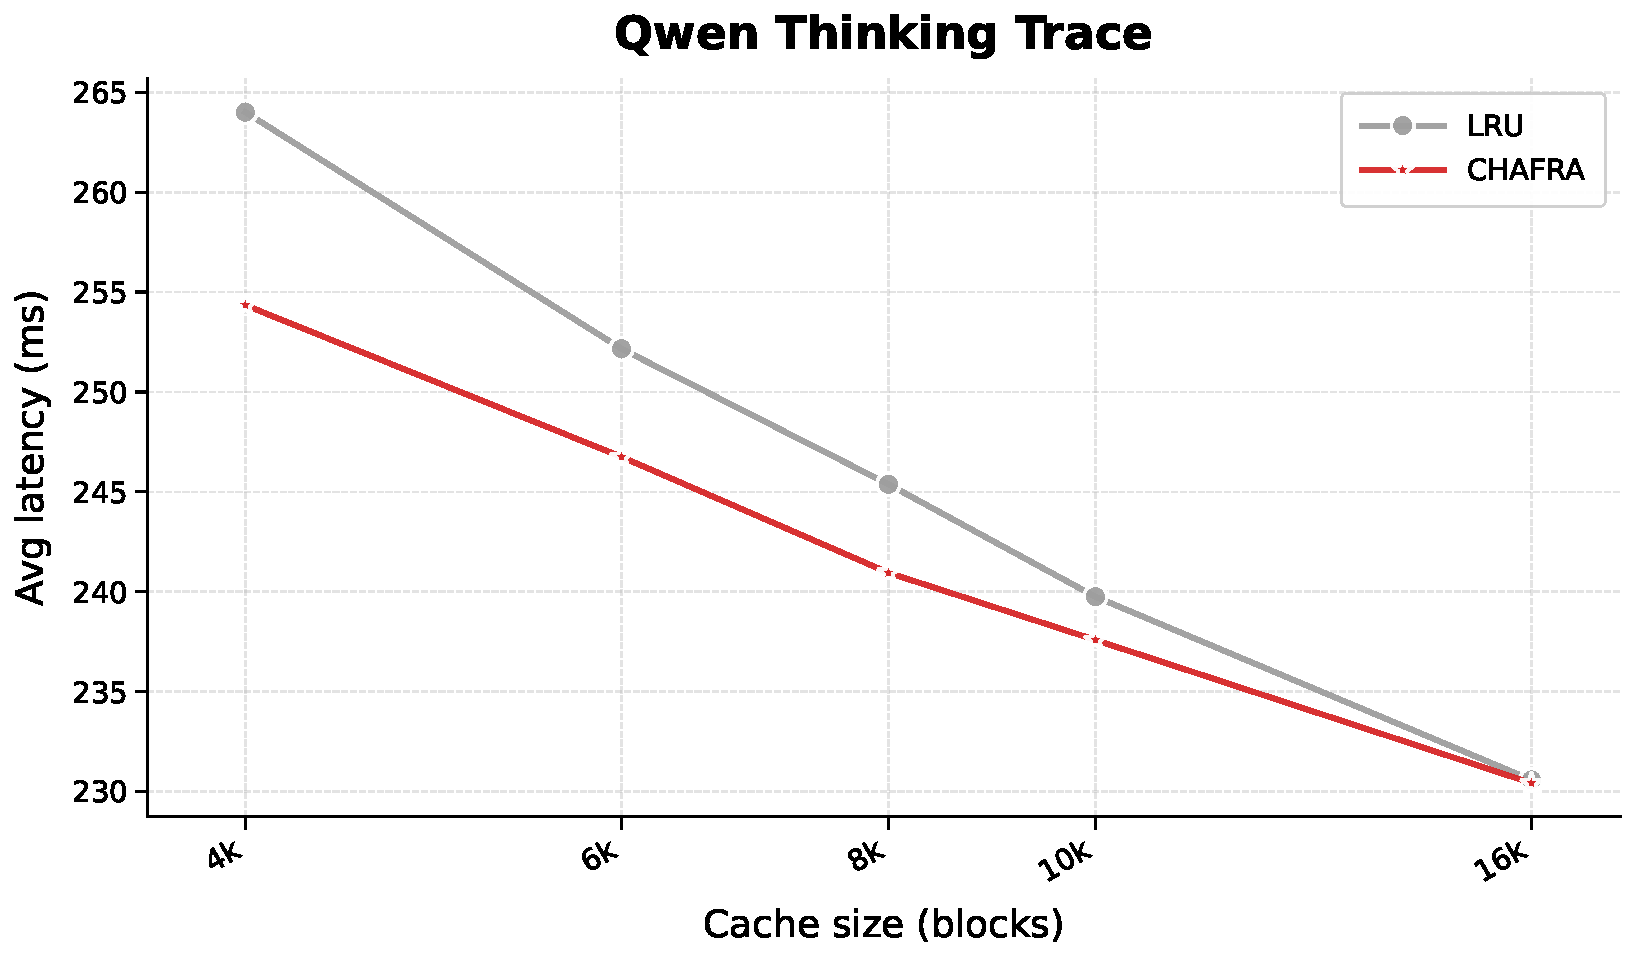
\includegraphics[width=\linewidth]{figure/qwen_thinking_blksz_16_pos_latency_pretty.pdf}
        \caption{Reasoning (Thinking)}
        \label{fig:latency-trace-thinking}
    \end{subfigure}
    \hfill
    \begin{subfigure}{0.48\textwidth}
        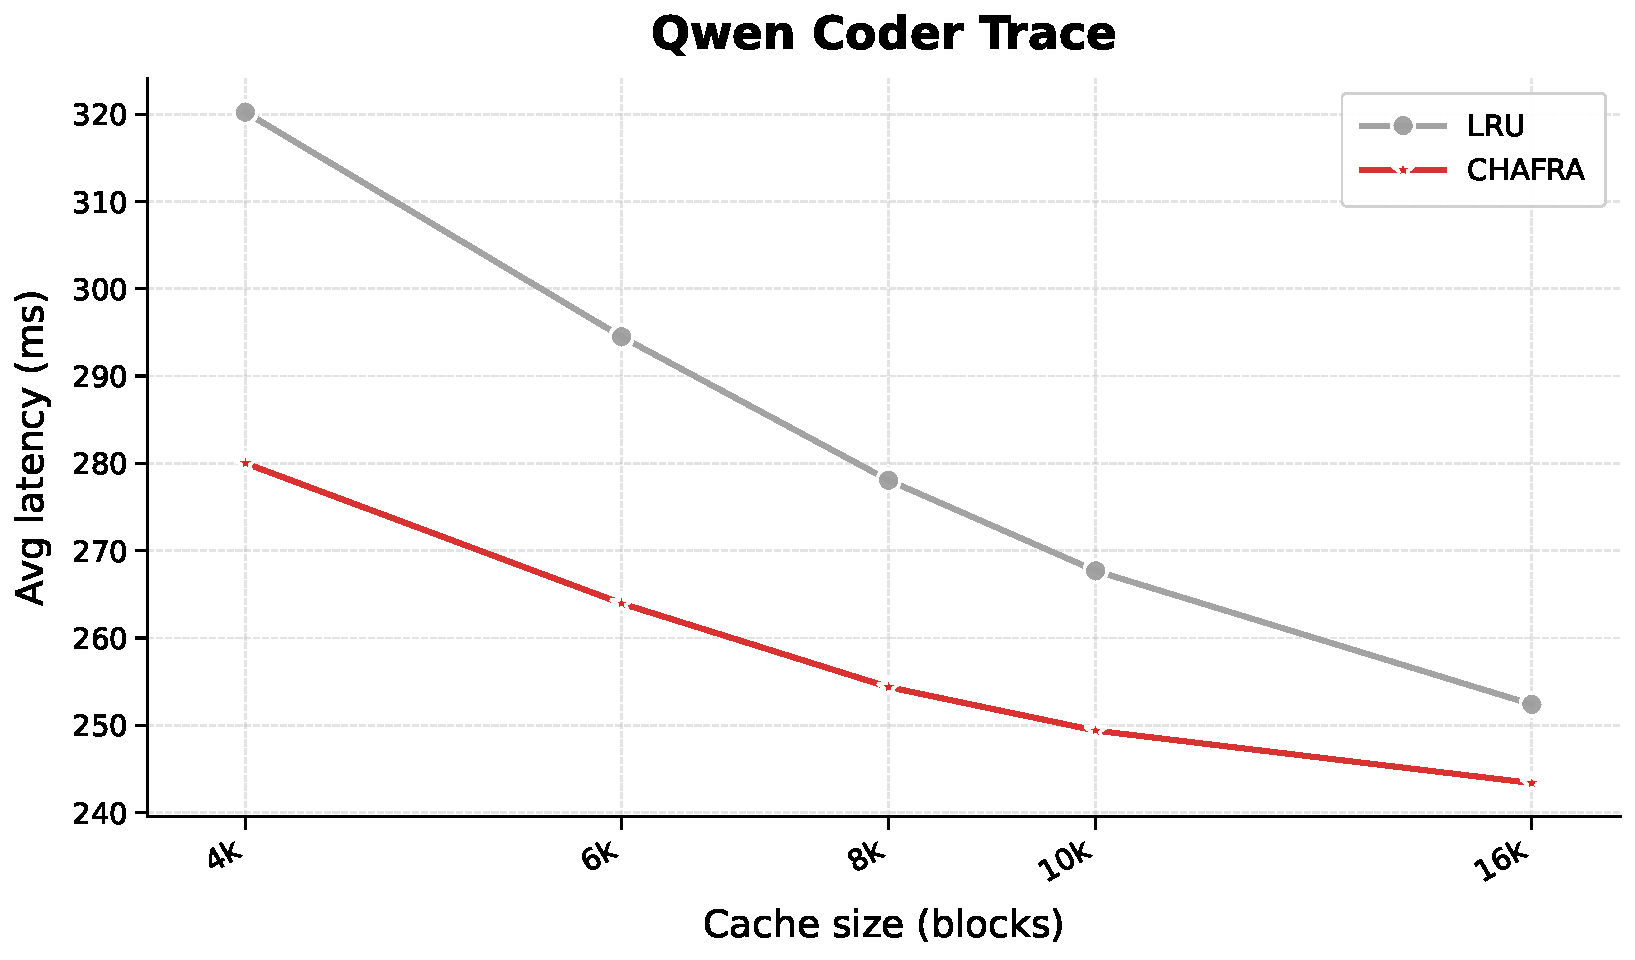
\includegraphics[width=\linewidth]{figure/qwen_coder_blksz_16_pos_latency_pretty.pdf}
        \caption{Coding Assistant (Coder)}
        \label{fig:latency-trace-coder}
    \end{subfigure}
    \caption{Average Time-to-First-Token (TTFT) for different eviction policies. By protecting deep prefix blocks, \sys significantly reduces the prefill latency compared to standard LRU.}
    \label{fig:qwen-latency-analysis}
\end{figure*}

The latency results strongly correlate with the computational savings observed in Section~\ref{sec:cache-analysis}. For workloads with high attention pressure, such as the coding assistant trace, \sys reduces the average TTFT by ensuring that the most expensive-to-recompute blocks remain cached. This optimization is critical for long-context serving, as it prevents the quadratic recomputation penalty that occurs when deep prefix blocks are evicted. Furthermore, the consistent performance of \algo across varying cache sizes demonstrates its robustness in maintaining low latency even under memory pressure.

Interestingly, we observe in certain traces that an extremely limited cache capacity (e.g., 4K blocks) may report a lower average TTFT than a slightly larger capacity (e.g., 6K blocks). This counter-intuitive trend is primarily due to request filtering: at very low capacities, the system is forced to skip or reject requests whose context lengths exceed the available physical memory. Since these skipped requests are precisely those that would incur the highest prefill latency, the resulting average TTFT only reflects shorter, less expensive queries. As the cache size increases (e.g., to 6K), the system begins to accommodate these longer requests, which naturally increases the overall average latency despite the larger cache providing more reuse opportunities.

\section{Conclusion}

In this project, we have presented \sys (\sysfull), a system designed to address the computational bottlenecks of prefix caching in long-context LLM serving. By recognizing that the recomputation cost of a KV cache block scales quadratically with its position in the sequence, we introduced the \algo (\algofull) algorithm. Unlike traditional eviction policies, \algo explicitly prioritizes the retention of deep, high-cost blocks, thereby minimizing the Time-to-First-Token (TTFT) and overall computational overhead.

Furthermore, we developed a hole-aware management system that handles the fragmentation inherent in block-level cache eviction. By implementing a batched hole-filling mechanism, \sys enables the efficient reuse of non-contiguous cached segments without incurring the scheduling penalties typical of sequential recomputation. Our evaluation across diverse production traces confirms that \sys significantly outperforms standard LRU-based policies and closely approximates the performance of offline optimal strategies. As LLM context windows continue to expand, the transition from simple cache-hit optimization to computation-aware caching will be essential for maintaining high-performance serving infrastructures.


\bibliographystyle{plain}
\bibliography{reference}
\end{document}
